Here we investigate the graphing capabilities of Mathcad.

\section{Mathcad: Graphing}\label{sec:Mathcadplots}

\index{Mathcad!Toolbars!Graphing}
Graphing is a great way for interpreting technical and scientific data. Two areas will be
discussed: 1) graphical presentation of data, 2) graphical analysis. Mathcad provides several
graphing options.\\
\\
The easiest way to begin a plot is to use the graphing toolbox.\\
OR\\
Use the menu options Insert/Graph/X-Y Plot\\
OR\\
Shortcut [Shift + 2]\\

The toolbar looks like \\
\\
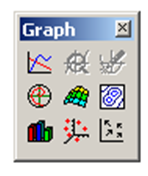
\includegraphics{figures/mathcad_plot_toolbar.png}\\

and clicking on the first button creates a blank plot\\
\\
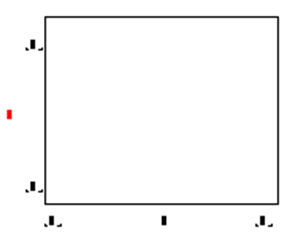
\includegraphics{figures/mathcad_blank_plot.png}\\

There are six place holders in the empty graph. The centered place holders are used for
$x$-coordinate and $y$-coordinate data and the other four are for the $x$ and $y$ bounds.\\

\example{ex_mathcadplot}{\po\\
\\
An engineer is testing a new material to find its modulus of elasticity, defined as the stress over the strain (or N/m). Plot the
data given $F$ vs. $\delta$.\\
\\
\tnr{F :=}
$
\left(
\begin{array}{c}
2\\
4\\
6\\
8\\
10\\
12\\
14\\
16\\
18\\
20
\end{array}
\right) 
\cdot \tnr{kN}
\qquad 
\delta :=
\left(
\begin{array}{c}
0.82\\
1.47\\
2.05\\
3.37\\
3.75\\
4.17\\
5.25\\
5.44\\
6.62\\
7.97
\end{array}
\right) 
\cdot$ \tnr{mm}\\
\\
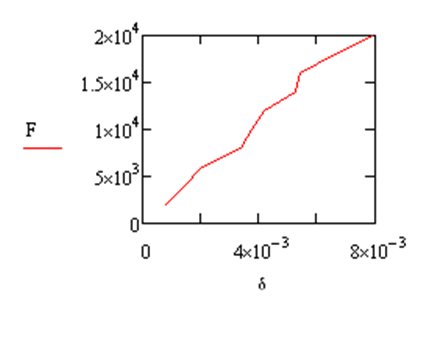
\includegraphics{figures/mathcad_Fdelta_plot.png}
}\\

If you wish to make any plot bigger, click on the plot. Grab the bottom right hand
handle with the mouse and drag it to make it larger.

If you want to reposition a plot, click on the plot, point to the outside edge of the area
until you see the hand, hold the mouse button down and drag the plot to a new location.

Note: Mathcad always plots in base units. So the plot in example \ref{ex_mathcadplot} is in Newtons for the $F$
and in meters for the $\delta$. Here we show the enlarged plot with the units removed. As you see the
plot now shows the values in the above tables with a unit on the axis. The center place
holders have the data value divided by the unit $F/kN$ and $\delta/mm$.\\

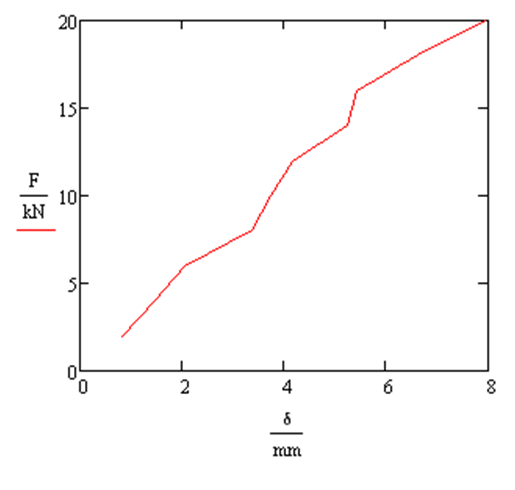
\includegraphics[scale=0.75]{figures/mathcad_Fdelta_plot2.png}

However, in example \ref{ex_mathcadplot} suppose we really want to see just the data points, not the connecting lines.  To do this, double click the graph to bring up the formatting dialog box.

\index{Mathcad!Plot Customization}
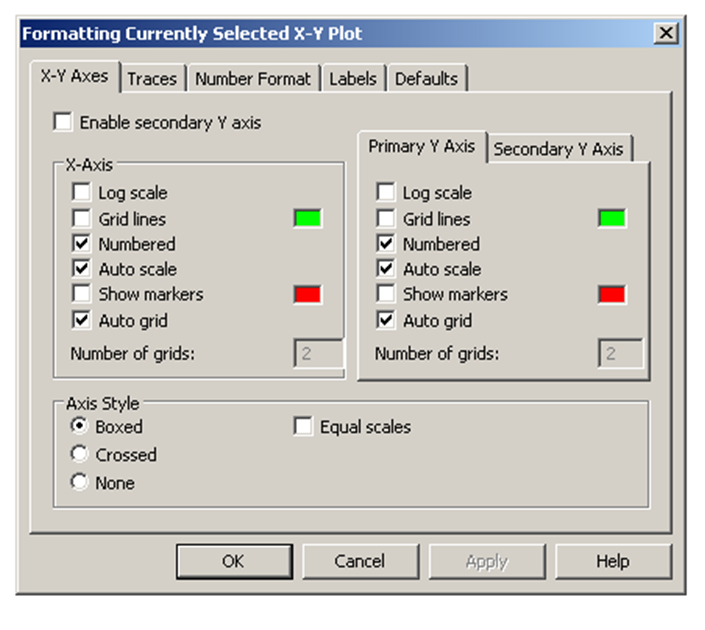
\includegraphics[scale=0.75]{figures/mathcad_Fdelta_plot3.png}\\

Go to the TRACES tab to add a symbol and remove the line. As you can see from the other tabs in this
dialog box, you make many changes to the way the graph is formatted.   A possible, reformatted graph appears below.\\
\\
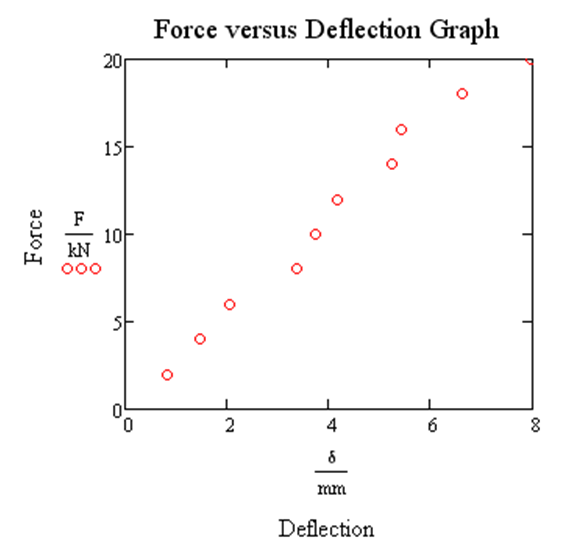
\includegraphics[scale=0.75]{figures/mathcad_Fdelta_plot4.png}\\

How about plotting multiple curves on the same plot?  We demonstrate this in the following example.\\  

\example{ex_mathcadmultiplot}{\po\\
\\
Begin by entering the data for the variables
\tnr{Time, Distance1} and \tnr{Distance2}.

\tnr{Time :=}
$
\left(
\begin{array}{c}
0\\
1\\
2\\
3\\
4\\
5\\
6
\end{array}
\right) 
\quad
\tnr{Distance1 :=}
\left(
\begin{array}{c}
0\\
4.9\\
19.6\\
44.1\\
78.4\\
122.5\\
176.4
\end{array}
\right)
\quad
\tnr{Distance2 :=}
\left(
\begin{array}{c}
5\\
19.8\\
76.8\\
153.3\\
256.2\\
394.5\\
559.2
\end{array}
\right)
$

Open a new plot and put \tnr{Time} in the $x$-axis.  For the $y$-axis, enter \tnr{Distance1} and then type a comma (important!!).  This will move you to a new line where you can type \tnr{Distance2}.  When you are done, click outside the graph to see the plot.  To customize the plot, double click the plot and use the Formatting dialog box.  See if you can match the plot below:

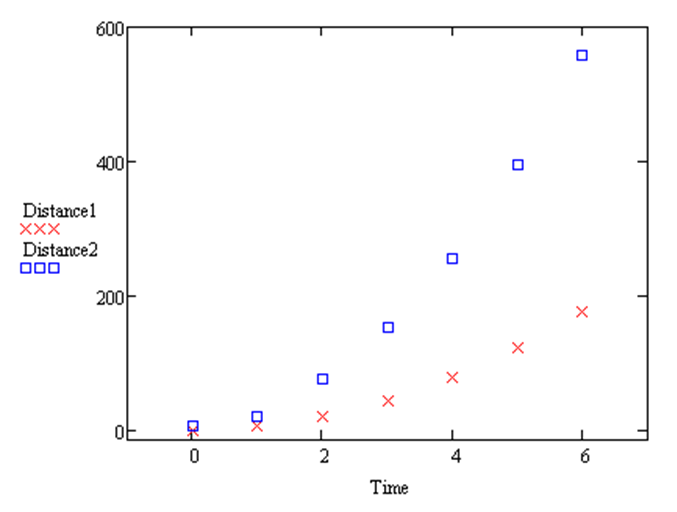
\includegraphics[scale=0.75]{figures/mathcad_multiple_plot.png}
}\\

\index{Mathcad!Quickplot}
If you want to see a plot of a predefined function, you can use a \textbf{Quickplot}.\\

\example{ex_quickplot}{\po \\
\\
Simply open a new plot, enter the variable $x$ on the $x$-axis and a function, say \tnr{sin(x)} on the $y$-axis.  The default plot has $x$ from -10 to 10.

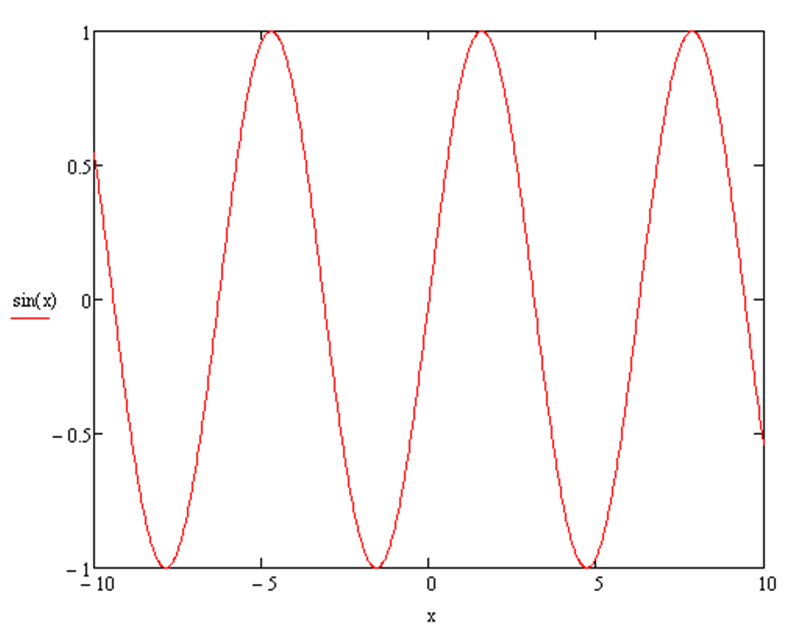
\includegraphics[scale=0.75]{figures/mathcad_sine_plot1.png}
}\\

In example \ref{ex_quickplot} if you want to change the $x$ values, first single click on the plot.  The numbers -10 and 10 appear at the bottom.  One at a time simply click on them and type in the new values 0 and $2 \pi$ (using the Greek toolbar).

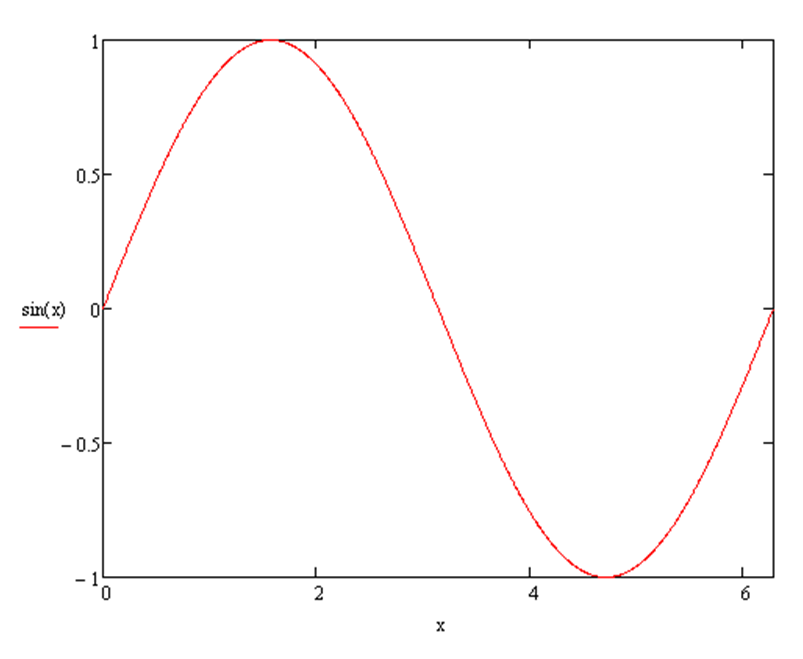
\includegraphics[scale=0.75]{figures/mathcad_sine_plot2.png}

Now for a more advanced example...\\

\example{ex_mathcadvibrationplot}{\po \\
\\
Here is the vibration response of a damped signal of freedom system to a step input.\\

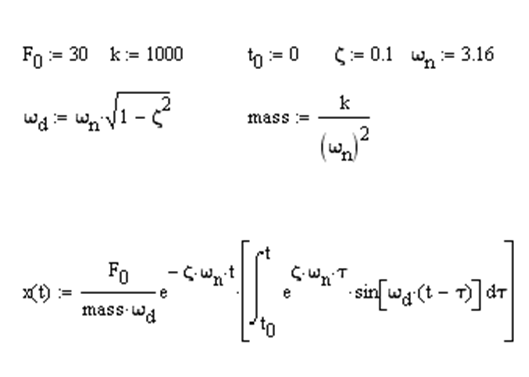
\includegraphics{figures/mathcad_damped_plot_def.png}

with resulting plot:

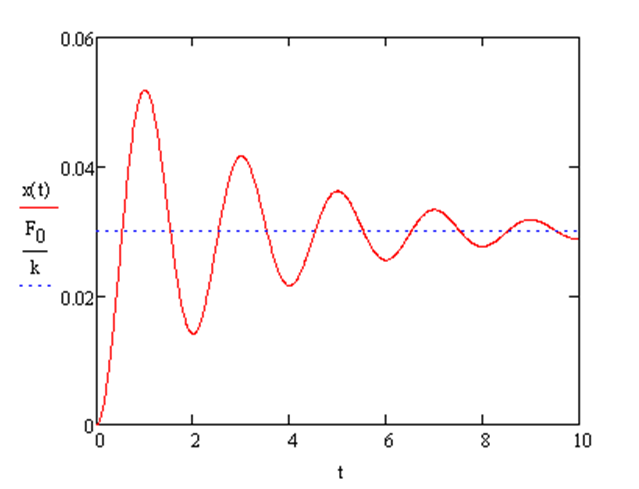
\includegraphics[scale=0.75]{figures/mathcad_damped_plot.png}
}\\

The last example may be difficult to reproduce.  Mastering how to input all of these parts into Mathcad takes time.  Be patient.

\newpage
\printexercises{exercises/15_exercises}